\begin{figure*}[t]
\centering
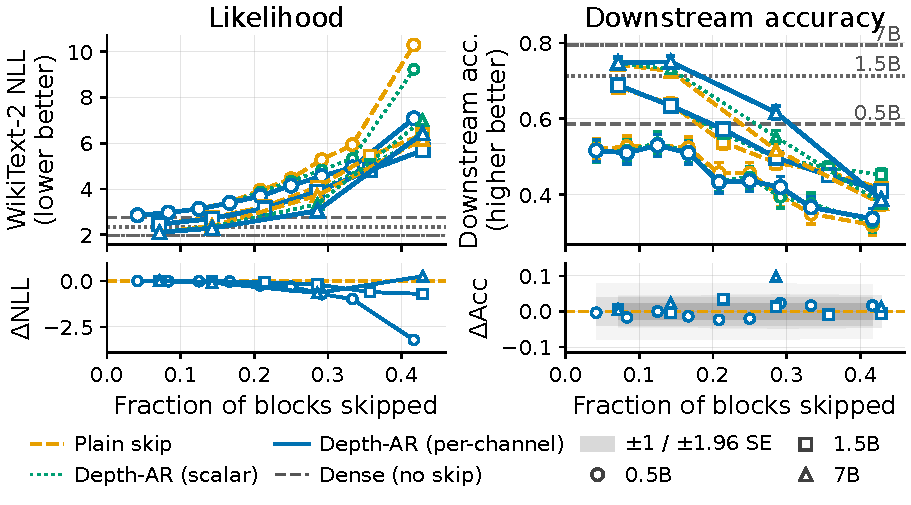
\includegraphics[width=0.62\textwidth]{figures/fig2_dissociation.pdf}
\caption{\textbf{Significant gains appear only where skipping does severe damage.} Quality against
the fraction of blocks skipped, for Qwen2.5-0.5B (circles), 1.5B (squares) and 7B (triangles),
with layers chosen by measured residual damage and every predictor skipping the identical
blocks. Lower panels plot the difference against plain skipping directly, so a point below zero
on the left is an improvement in likelihood and a point above zero on the right is an
improvement in accuracy. Shaded bands are $\pm 1$ and $\pm 1.96$ binomial standard errors.
Where skipping barely hurts, at the left of each panel, \mname and plain skipping are
indistinguishable in behaviour, and the differences there are smaller than the evaluation's own
measured reproducibility floor. Where skipping does severe damage the gap opens: at 28.6\% of
blocks skipped on 7B, \mname answers 89 more questions correctly out of 900 than plain skipping
($z=4.31$, surviving Bonferroni correction across all 63 comparisons) while recovering 38.1\%
of its language-modelling damage. Both breakdowns are drawn rather than hidden: at 42.9\%
skipped on 7B the depth-only predictor falls \emph{below} plain skipping on likelihood, where
the cross-token extension does not. Hardware and protocol: \Cref{sec:app-protocol}.}
\label{fig:dissociation}
\end{figure*}
